\documentclass[10pt]{book}
\usepackage{commands}

\usepackage{bbm}


\begin{document}




\begin{tikzpicture}[remember picture,overlay]
	% If a chapter image has been specified
	\expandafter\ifstrequal\expandafter{\thechapterimage}{}{}{
		% Output the chapter image
		\node[
		anchor=north west, % Anchor point on the image
		inner sep=0pt, % Inner padding
		] at (current page.north west) {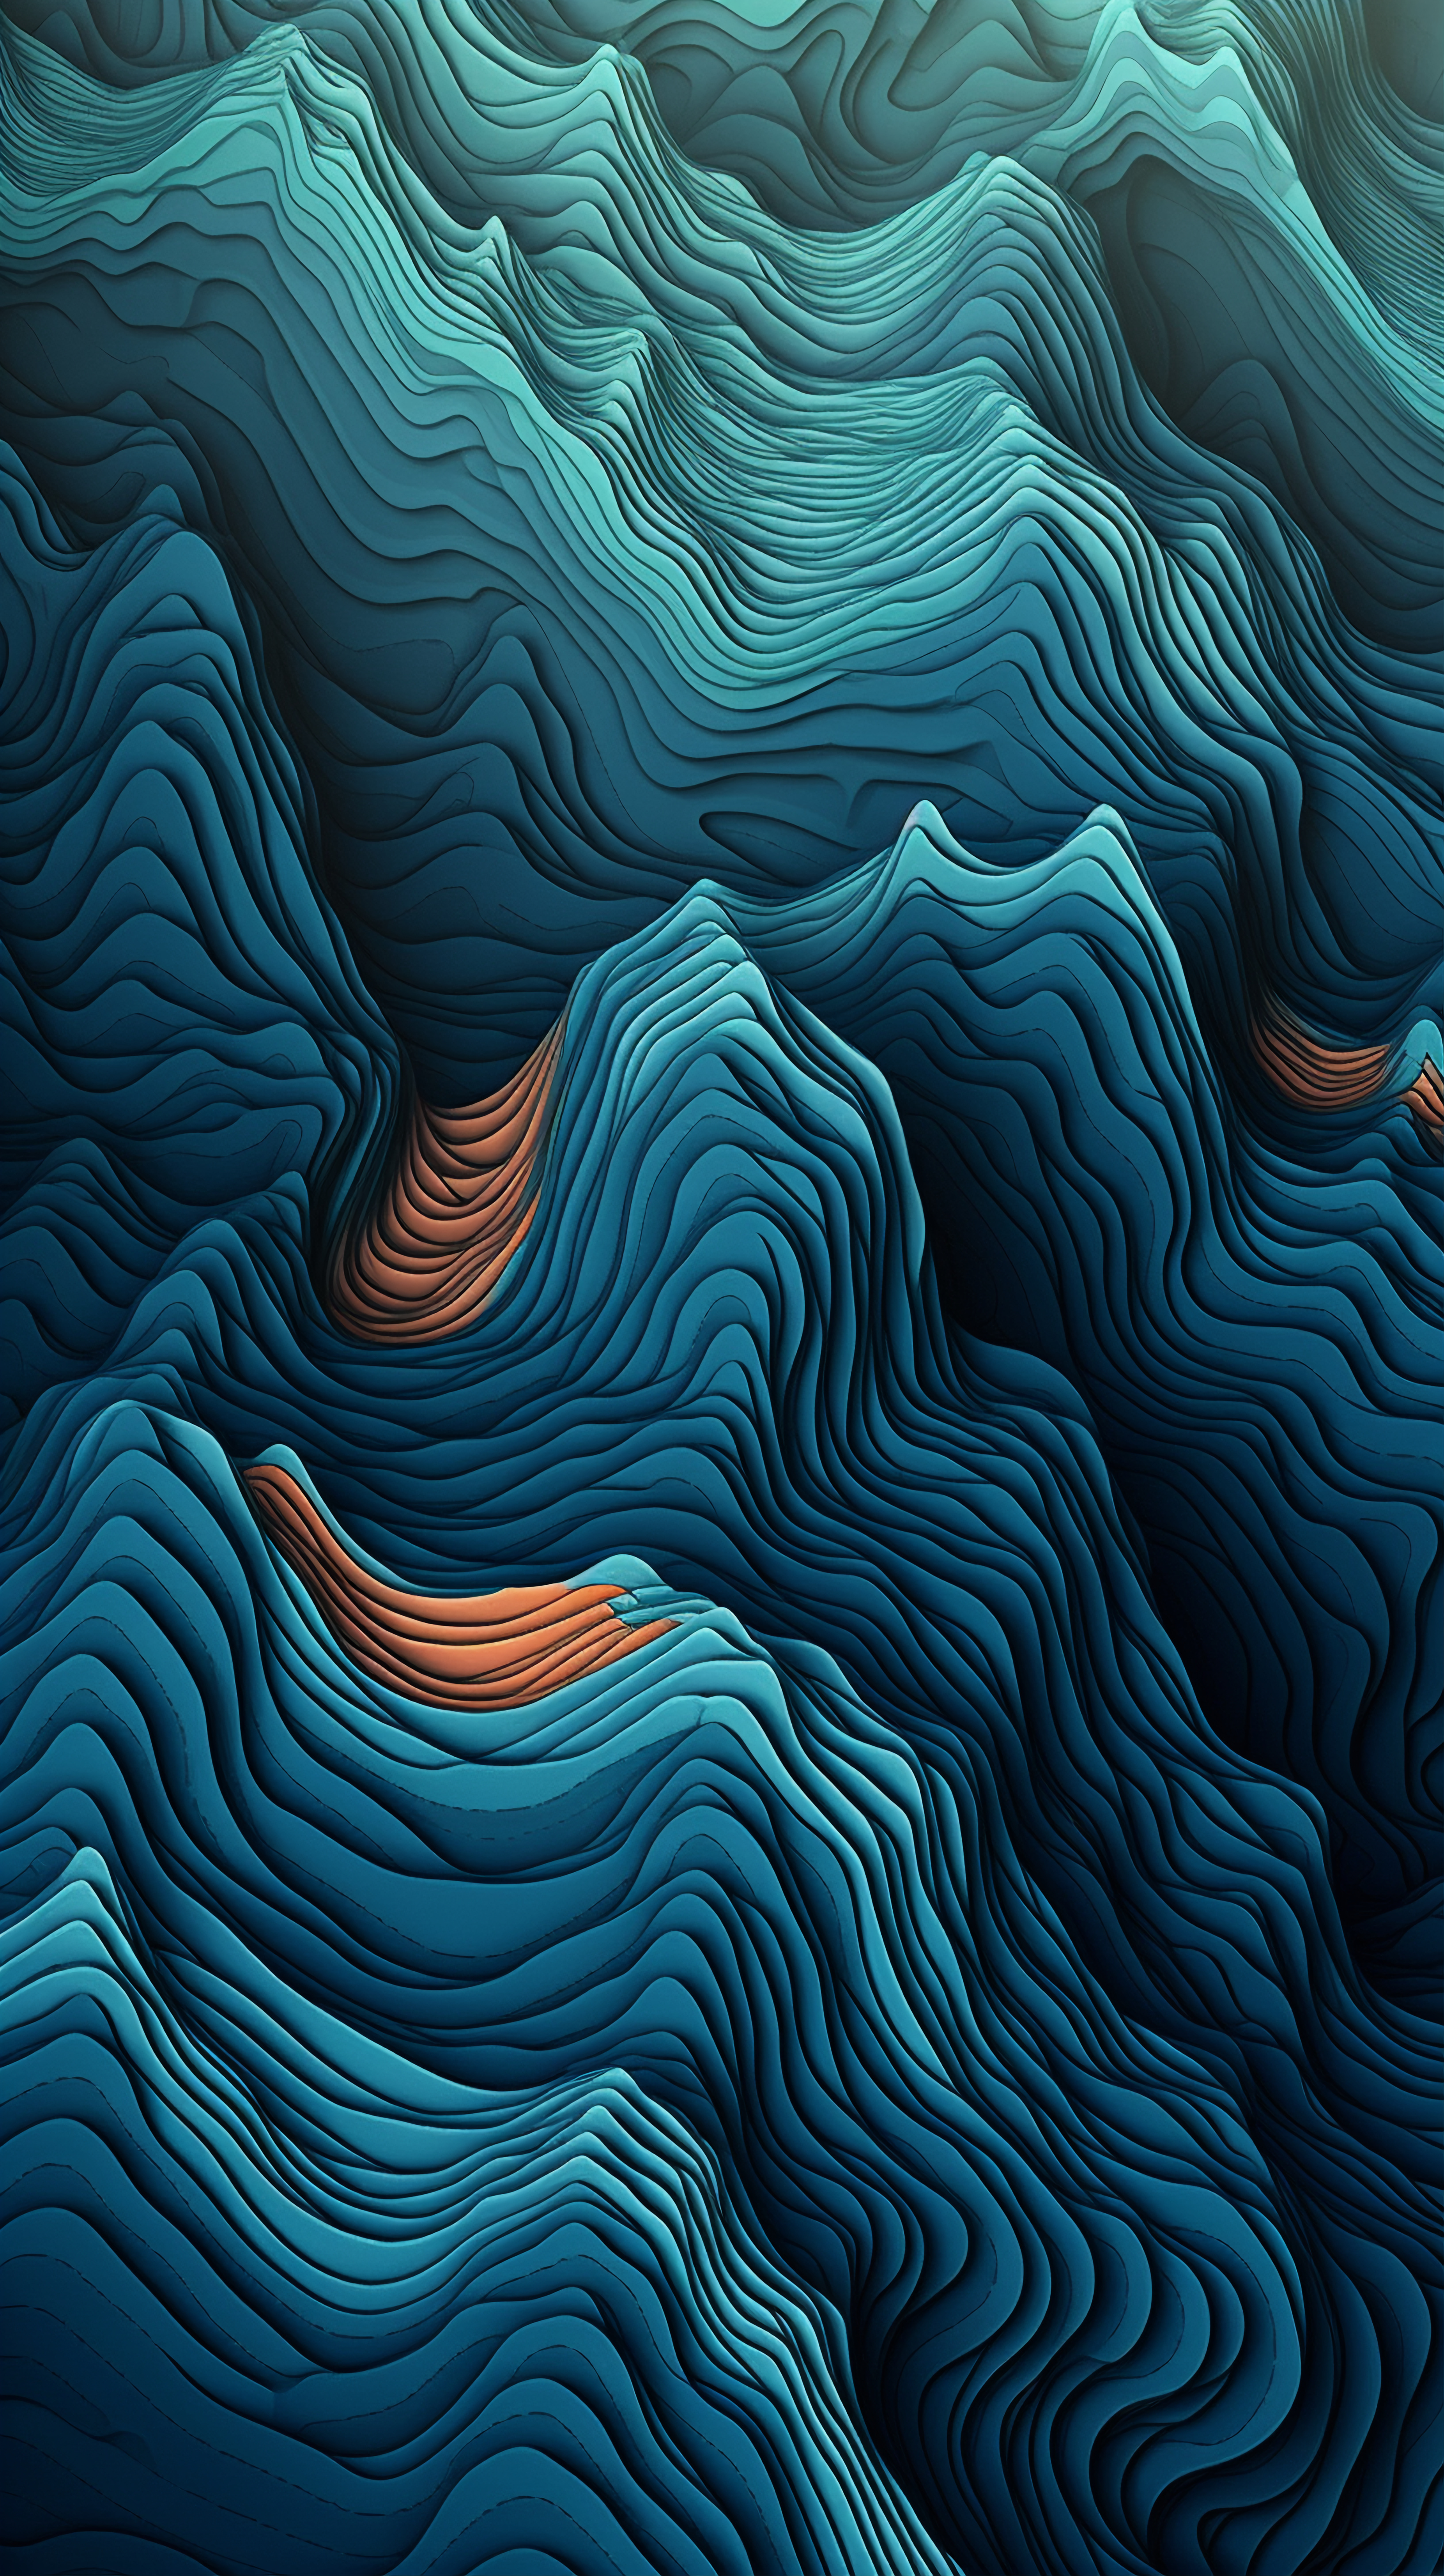
\includegraphics[angle=0,height=\paperheight]{Images/output}};
	}
\end{tikzpicture}

\vspace{3cm}

\heading{Daily Notes}


%\begin{figure}[h!]
%	\centering
%	\includegraphics[width=1\linewidth]{Images/realAnalysis}
%	\caption*{$\mathbb{R}$eal Analysis, Created by DALL-E!}
%	\label{fig:realanalysis}
%	
%\end{figure}




\tableofcontents

\chapter{Manifolds}

\begin{quote}
	{\color{orange} \textbf{Very important note:}} Throughout this text, to avoid repeating some words like \emph{smooth,  and etc}, we often omit them and we let the context to reflect these notions. So we emphasis that throughout this text, unless otherwise specified, by a \textbf{manifold} we always mean a $ C^\infty $ manifold. An atlas of a chart on a smooth manifold means an atlas or a chart contained in the differentiable structure of the smooth manifold.
\end{quote} 


\section{Topological manifolds and Smooth manifolds}

We start with the definition of topological manifolds. We will later study the smooth manifolds that are of our main interest in this lecture. But first, we need to review some basic definition.

\begin{definition}[Hausdorff topological space]
	A set $ A $, along with a collection of subsets of $ A $ called $ \mathcal{T} \subset 2^A $, i.e. $ (A,\mathcal{T}) $ is called a topological space if we have
	\begin{enumerate}[(I)]
		\item $ \emptyset \in \mathcal{T} $ and $ A \in \mathcal{T} $.
		\item For any infinite collection $ \set{A_\alpha}_\alpha \subset \mathcal{T} $ we have
		\[ \bigcup_{\alpha} A_\alpha \in \mathcal{T}. \]
		\item For a finite collection $ \set{A_i}_{i \in I} $ where $ I = \set{1,2,\cdots,N} $ for some $ N \in \N $, we have
		\[ \bigcap_{i \in I} A_i \in \mathcal{T}. \]
		\item $ \forall x,y \in A $ there exists $ U,V \in \mathcal{T} $ such that $ x\in U $ and $ y \in V $ and we have $ U \cap V = \emptyset $.
	\end{enumerate}
\end{definition}


The following definition reviews the notion of second countable topological spaces.

\begin{definition}[Second countable topological spaces]
	Let $ (X,\mathcal{T}) $ be a topological space. This space is second countable if there exists an at most countable collection of sets $ \mathcal{B} \subset \mathcal{T} $ such that $ \forall U \in \mathcal{T} $ we have
	\[ U = \bigcup_{A \in \mathcal{B}} A. \]
	I.e. any open set in $ \mathcal{T} $ can be written as a union of sets in $ \mathcal{B} $
\end{definition} 

The last piece of definition that we need is the notion of locally Euclidean spaces.

\begin{definition}[Locally Euclidean topological spaces]
	Let $ (X,\mathcal{T}) $ be a topological space. We say $ X $ is locally Euclidean if $ \forall p \in X $, there exists an open neighborhood $ p \in U \in \mathcal{T}$ such that is homeomorphic to an \emph{open} subset of $ \R^n $. I.e. there is a homeomorphism $ \phi: U \to \R^n $. We call the pair $ (U,\phi:U\to\R^n) $ a \emph{chart}, $ U $ a \emph{coordinate neighborhood} or a \textbf{coordinate open set}, and $ \phi $ a \emph{coordinate map} or \emph{coordinate system} on $ U $. 
\end{definition}


\begin{definition}[Topological manifolds]
	A topological manifold is a Hausdorff, second countable topological space that is locally Euclidean space. It is said to be of dimension $ n $, if it is locally Euclidean of dimension $ n $.
\end{definition}


In the following section, we will review the notion of compatible charts which will be central to our study of manifolds. Assume we have two charts $ (U,\phi) $ and $ (V,\psi) $. Since $  U,V $ are open in $ M $ (the manifold), then $ U\cap V $ is open in $ U $ and $ V $. Furthermore, since $ \phi $ is a homeomorphism to an open subset of $ \R^n $ then $ \phi(U\cap V) $ and $ \psi(U\cap V) $ are also open. One way to show this, let $ \phi(U cap V) = B, \phi(U) = A, $ and $ A\backslash B = C $. We know that $  A $ is open, and $ B\cup C = A, B \cap C = \emptyset $. Then $ A $ being open implies $ B $ and $ C $ is open. Now we can make the following definition for $ C^\infty $-compatible maps.

\begin{definition}[$ C^\infty $ compatible maps]
	Let $ M $ be a topological manifold, where $ (U,\phi) $ and $ (V,\psi) $ are two charts. These charts are called $ C^\infty $-compatible if the maps
	\[ \phi\circ \inv{\psi} : \psi(U\cap V) \to \phi(U\cap V)\qquad \text{and} \qquad  \psi \circ\inv{\phi}: \phi(U \cap V) \to \psi(U\cap V),  \]
	are $ C^\infty $. These two maps are called \emph{transition functions} between charts. 
\end{definition}

\begin{remark}
	If two $ U,V $ in the definition above, i.e. $ U\cap V = \emptyset $, then they are automatically compatible.
\end{remark}

\begin{definition}[$ C^\infty $ atlas]
	Let $ M $ be a topological manifold. The collection of charts $ \mathcal{U} = \set{(U_\alpha, \phi_\alpha)} $ is called a $ C^\infty $ atlas, or simply an atlas if 
	\begin{itemize}
		\item all of the charts are pairwise $ C^\infty $ compatible,
		\item the charts cover the whole manifold, i.e. $ M = \bigcup_\alpha U_\alpha $.
	\end{itemize}
\end{definition}

\begin{lemma}
	Let $ \mathcal{A} = \set{(U_\alpha,\phi_\alpha)}_{\alpha \in I} $ be an atlas for the manifold $ M $. Let $ (V,\psi) $ and $ (W,\sigma) $ be two charts where both of them are compatible with the atlas $ \mathcal{A} $. Then these two charts are compatible with each other.
\end{lemma}

\begin{proof}
	We start by showing that $ \psi\circ \inv{\sigma} $ is $ C^\infty $ on $ V\cap W $. Let $ p \in V \cap W $. Then $ \exists \alpha \in I $ such that $ p \in U_\alpha $ for the chart $ (U_\alpha,\phi_\alpha) $. Then 
	\[ (\psi \circ \inv{\phi_\alpha})\circ (\phi_\alpha \circ \inv{\sigma}): \sigma(W\cap U_\alpha \cap V) \to \psi(W \cap U_\alpha \cap V) \]
	is $ C^\infty $ in $ \sigma(W\cap U_\alpha \cap V) $, because it is the composition of $ C^\infty $ maps. Call $ \mathbb{B}_\alpha  = W\cap U_\alpha \cap V $. Then what we have shows is simply $ \forall p \in V \cap W $, there exists an open set $ p \in \mathbb{B}_\alpha \subset V\cap W $ for $  \alpha \in I $ and the map $ \psi \circ \inv{\sigma}  $ is $ C^\infty $ in $ \mathbb{B}_\alpha $. Since this holds for every $ p \in V \cap W $ this proves that $ \psi\circ \inv{\sigma} $ is $ C^\infty $ on $ \sigma (V\cap W) $. Similarly, we can show $ \sigma \circ \inv{\psi} $ is $ C^\infty $ on $ \psi(V\cap W) $, and this completes the proof.
\end{proof}

\begin{remark}
	Note that in an equality like $ \psi \circ \inv{\sigma} =(\psi \circ \inv{\phi_\alpha})\circ (\phi_\alpha \circ \inv{\sigma}) $, two functions in the sides of the equality have different domains. So the equality sign here means that these two functions are equal on their common domain.
\end{remark}


\begin{definition}[Maximal atlas]
	Let $ \mathcal{U} $ be an atlas for the manifold $ M $. Then $ \mathcal{U} $ is called maximal if it contains any other atlas of the manifold $ M $. Or equivalently, if $ \mathcal{M} $ is any other atlas containing $ \mathcal{U} $ then $ \mathcal{U} = \mathcal{M} $.
\end{definition}

We can use the notion of the maximal atlas to define a smooth manifold.

\begin{definition}[Smooth manifold]
	A topological manifold together with a maximal atlas is called a smooth manifold. The maximal atlas is also called a differentiable structure on $ M $.
\end{definition}


In practice, to show that a topological manifold is smooth, it is not necessary to exhibit a maximal atlas. Existence of any atlas will do so, as proposed by the following proposition.


\begin{proposition}
	Any atlas of a locally euclidean space is contained in a \emph{unique} maximal atlas.
\end{proposition}

\begin{proof}
	Let $ \frak{U} = \set{(U_\alpha, \phi_\alpha)} $ be any atlas for the locally Euclidean space $ M $. Let $ S = \set{(V_i, \psi_i)} $ denote the set of all charts compatible with $ \frak{U} $. Construct the set $ \frak{M} = \frak{U} \cup S $. We claim that this set is a maximal atlas. Let $ (W,\psi) $ be a chart compatible with $ \frak{M} $. Then it should also be compatible with $ \frak{U} $, thus it is contained in the set $ S $, i.e. $ (W,\psi) \in S $, thus in $ \frak{M} $. This shows that the atlas $ \frak{M} $ is maximal.
	
	To show the uniqueness, let $ \frak{M}' $ be another maximal atlas. Since $ \frak{M}' $ is compatible with $ \frak{U} $, thus it is also compatible with $ \frak{M} $. But due to the construction it is contained in the new atlas, thus $ \frak{M}' \subset \frak{M} $. Thus the maximal atlas is unique.
\end{proof}

Considering the proposition above, we arrive at the following important observation.

\begin{observation}[Showing a space is an smooth manifold]
	To show that a space is an smooth manifold, we just need to show that the space is
	\begin{itemize}
		\item a Hausdorff topological space that is also second countable,
		\item there exists any $ C^\infty $ atlas (not necessarily maximal).
	\end{itemize}
\end{observation}


\section{Smooth maps on a manifold}
In this section, we will study the notion of smooth maps between manifolds. We will use the notion of coordinate charts to transfer the notion of smooth maps from Euclidean spaces to manifolds. We start with the functions on manifolds.

\begin{definition}[Smooth functions on manifolds]
	Let $ f:M \to R $ be a function on a manifold. The function $ f $ is smooth at point $ p \in M $ if there exists a chart $ (U,\phi) $ such that $ p \in U $ and the map
	\[ f \circ \inv{\phi}\ :\ \phi(U) \to \R \]
	is smooth at $ p $. The function $ f $ is said to be $ C^\infty $ on $ M $ if it is $ C^\infty $ at every point of $ M $.
\end{definition}
\begin{remark} 
	Note that the smoothness of the function $ f $ in the definition above is independent of the local chart $ (U,\psi) $ that we choose. Let $ (V,\psi) $ be another local chart containing the point $ p $. Then the map $ f \circ \inv{\psi} $ is also smooth at $ p $. Because
	\[ f \circ \inv{\psi}: (f\circ \inv{\phi}) \circ (\phi \circ \inv{\psi}). \]
	We know that the map $ (\phi \circ \inv{\psi} $ is smooth at $ p $ (since the local charts in an atlas are compatible). Also $ (f\circ \inv{\phi}) $ is smooth (we have assumed so). Thus $ f \circ \inv{\psi} $ is smooth.
\end{remark}

\begin{proposition}[Smoothness of real valued functions]
	Let $ M $ be a manifold of dimension $ n $ with atlas $ \frak{U} $, and let $ f: M \to \R $ a real-valued function on $ M $. The following are equivalent:
	\begin{enumerate}[(i)]
		\item The function $ f : M \to \R $ is $ C^\infty $.
		\item The manifold $ M $ has an atlas such that for every chart $ (U,\phi) $ in the atlas, $ f\circ \inv{\phi}: \phi(U) \to \R$ is $ C^\infty $.
		\item For every chart $ (V,\psi) $ on $ M $, the function $ f\circ \inv{\psi}: \psi(V) \to \R $ is $ C^\infty $.
	\end{enumerate}
\end{proposition}

\begin{proof}
	We prove a cyclic chain of implications $ (ii)\implies (i) \implies (iii) \implies (ii) $.
	
	\noindent $ (ii) \implies (i) $: Let $ p \in M $. From the assumption we know that there is an atlas with the desired property. Thus $ \exists (U_\alpha,\phi_\alpha)  $ that contains $ p $ and the function $ f\circ\inv{\phi}: \phi(U) \to \R $ is smooth. 
	Thus $ f:M\to \R $ is smooth at $ p $, ans since the point $ p $ was arbitrary, then $ f $ is smooth on $ M $.
	
	\noindent $ (i) \implies (iii) $: Let $ p \in U $. From assumption we know that there is a coordinate open set $ U_\alpha $ such that $ f \circ \inv{\phi_\alpha}: \phi_\alpha(U)\to \R $ is smooth. Then we can write
	\[ f\circ\inv{\psi} = (f\circ\inv{\phi_\alpha})\circ(\phi_\alpha \circ \inv{\psi}) \]
	which shows that $ f\circ\inv{\psi}  $ is smooth (look at the remark below).
	
	\noindent $ (iii) \implies (ii) $: This follows immediately from the definition.
\end{proof}

%\begin{quote}
%	{\color{orange} I am not sure about the remark below. I need to discuss this with Ata in one of our weekly meetings$\ \Downarrow\Downarrow\Downarrow\Downarrow$.}
%\end{quote}
%\begin{remark}
%	Note that when we are saying ``let $ M $ be a manifold of dimension $ n $'' (in the first part of the proposition), what we really means is that the set $ M $ along with the collection of compatible charts (i.e. atlas) $ \frak{U} $ forms a manifold. In the part (iii) of the proposition above, when we say ``for every chart $ (V,\phi) $'' on manifold $ M $, what we really mean is $ (V,\phi) $ is compatible with $ \frak{U} $.
%\end{remark}

\begin{remark}
	Considering the ``very important note'' at the beginning of this chapter, we need to emphasis again that in part $ (iii) $, when we say \emph{for every chart $ (V,\psi) $ on $ M $}, we mean a chart in the unique differentiable structure of the manifold that contains the atlas $ \frak{U} $.
\end{remark}

\begin{observation}[From W. Tu]
	The smoothness conditions from the proposition above will be a recurrent motif through out the book. To prove the smoothness of an object, it is sufficient that a smoothness criterion hold on the charts of some atlas. Once the object is shown to be smooth, it then follows that the same smoothness criterion holds on every chart on the manifold.
\end{observation}


\begin{definition}[Pull back of a function]
	Let $ F: N\to M $ be a a map between manifolds, and $ \phi: M \to \R $. Then the pullback of the function $ \phi $ by $ F $ is denoted by $ F*\phi $ is defined as 
	\[ F^* \phi = \phi\circ F. \]
\end{definition}

\begin{remark}
	In this terminology, a function $ f:M \to \R $ is smooth on a chart $ (U,\phi) $ if and only if the pullback $ (\inv{\phi})^* f$ is smooth on the subset $ \phi(U) $ of Euclidean space.
\end{remark}

\subsection{Smooth maps between manifolds}
Here in this section we will discuss the smooth maps between manifolds. We will be able to recover the definition of the smooth functions on manifolds as a special case. 

\begin{definition}[Smooth maps between manifolds]
	Let $ M, N $ be manifolds with dimensions $ m,n $ respectively. A map $ F: M \to N $ is said to be smooth at point $ p \in M $, if there exists charts $ (U,\phi) $ and $ (V,\psi) $ such that $ p \in U $ and $ F(p) \in V $, and the function 
	\[ \psi\circ F \circ \inv{\phi}: \R^m \supset \phi(\inv{F}(V) \cup U) \to \R^n  \]
	is smooth at $ p $. The map $ F $ is said to be smooth on manifold $ M $ if it is smooth at every point of the manifold.
\end{definition}
\begin{remark}
	The following figure helps to digest the definition above.
	\begin{figure}[h!]
	\centering
	
	
	
	
	
	\tikzset{every picture/.style={line width=0.75pt}} %set default line width to 0.75pt        
	
	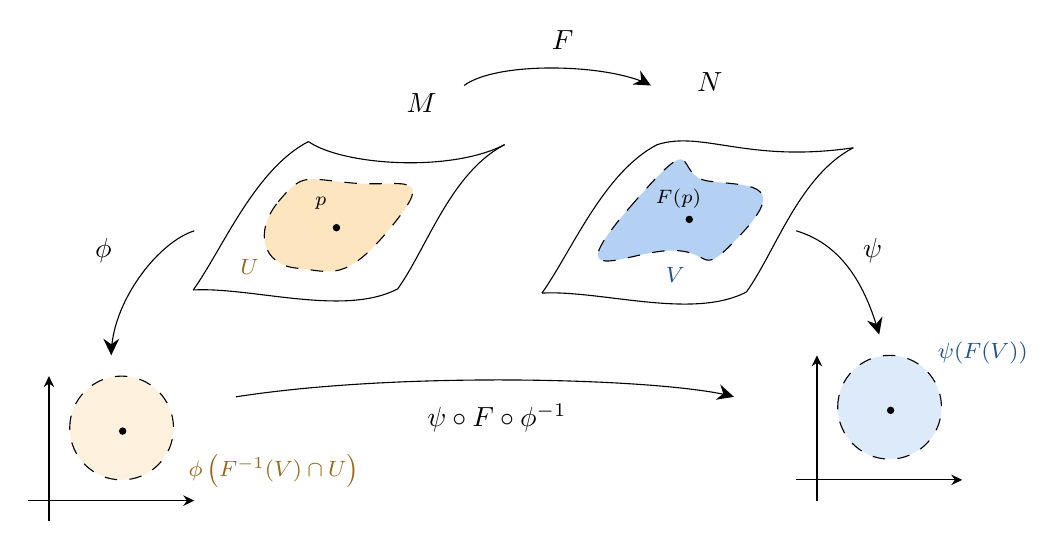
\begin{tikzpicture}[x=0.75pt,y=0.75pt,yscale=-1,xscale=1]
		%uncomment if require: \path (0,300); %set diagram left start at 0, and has height of 300
		
		%Curve Lines [id:da11806081372332144] 
		\draw    (179.5,178.5) .. controls (193.5,159) and (209,120.5) .. (235,107) ;
		%Curve Lines [id:da18965221151827483] 
		\draw    (179.5,178.5) .. controls (208,177) and (252,191.5) .. (278,178) ;
		%Curve Lines [id:da4778597706036809] 
		\draw    (278,178) .. controls (292,158.5) and (303.5,122) .. (329.5,108.5) ;
		%Curve Lines [id:da40033578881982557] 
		\draw    (235,107) .. controls (251.5,118.5) and (303.5,122) .. (329.5,108.5) ;
		%Curve Lines [id:da8289769291382043] 
		\draw    (347.5,180) .. controls (361.5,160.5) and (377,122) .. (403,108.5) ;
		%Curve Lines [id:da562782587348567] 
		\draw    (347.5,180) .. controls (376,178.5) and (420,193) .. (446,179.5) ;
		%Curve Lines [id:da8325596531064072] 
		\draw    (446,179.5) .. controls (460,160) and (471.5,123.5) .. (497.5,110) ;
		%Curve Lines [id:da2852542457229288] 
		\draw    (403,108.5) .. controls (425,101.5) and (446.5,117.5) .. (497.5,110) ;
		%Shape: Polygon Curved [id:ds40810252904164956] 
		\draw  [fill={rgb, 255:red, 245; green, 166; blue, 35 }  ,fill opacity=0.29 ][dash pattern={on 4.5pt off 4.5pt}] (220.5,136) .. controls (232.5,121.5) and (233.5,125) .. (256.5,127) .. controls (279.5,129) and (297.5,120.5) .. (275,148) .. controls (252.5,175.5) and (246,169.5) .. (229.5,168) .. controls (213,166.5) and (208.5,150.5) .. (220.5,136) -- cycle ;
		%Shape: Polygon Curved [id:ds4832622018481927] 
		\draw  [fill={rgb, 255:red, 74; green, 144; blue, 226 }  ,fill opacity=0.41 ][dash pattern={on 4.5pt off 4.5pt}] (390,138.5) .. controls (425.5,97.5) and (410,123.5) .. (427.5,126) .. controls (445,128.5) and (467,126) .. (444.5,150.5) .. controls (422,175) and (431,159) .. (409.5,159.5) .. controls (388,160) and (354.5,179.5) .. (390,138.5) -- cycle ;
		%Straight Lines [id:da8425805433734557] 
		\draw    (110,223) -- (110,290) ;
		\draw [shift={(110,220)}, rotate = 90] [fill={rgb, 255:red, 0; green, 0; blue, 0 }  ][line width=0.08]  [draw opacity=0] (5.36,-2.57) -- (0,0) -- (5.36,2.57) -- (3.56,0) -- cycle    ;
		%Straight Lines [id:da3867027047624212] 
		\draw    (177,280) -- (100,280) ;
		\draw [shift={(180,280)}, rotate = 180] [fill={rgb, 255:red, 0; green, 0; blue, 0 }  ][line width=0.08]  [draw opacity=0] (5.36,-2.57) -- (0,0) -- (5.36,2.57) -- (3.56,0) -- cycle    ;
		%Shape: Circle [id:dp9021706695013989] 
		\draw  [fill={rgb, 255:red, 245; green, 166; blue, 35 }  ,fill opacity=0.15 ][dash pattern={on 4.5pt off 4.5pt}] (120,245) .. controls (120,231.19) and (131.19,220) .. (145,220) .. controls (158.81,220) and (170,231.19) .. (170,245) .. controls (170,258.81) and (158.81,270) .. (145,270) .. controls (131.19,270) and (120,258.81) .. (120,245) -- cycle ;
		%Straight Lines [id:da20897051537256983] 
		\draw    (480,213) -- (480,280) ;
		\draw [shift={(480,210)}, rotate = 90] [fill={rgb, 255:red, 0; green, 0; blue, 0 }  ][line width=0.08]  [draw opacity=0] (5.36,-2.57) -- (0,0) -- (5.36,2.57) -- (3.56,0) -- cycle    ;
		%Straight Lines [id:da4413765041127402] 
		\draw    (547,270) -- (470,270) ;
		\draw [shift={(550,270)}, rotate = 180] [fill={rgb, 255:red, 0; green, 0; blue, 0 }  ][line width=0.08]  [draw opacity=0] (5.36,-2.57) -- (0,0) -- (5.36,2.57) -- (3.56,0) -- cycle    ;
		%Shape: Circle [id:dp2483574720488635] 
		\draw  [fill={rgb, 255:red, 74; green, 144; blue, 226 }  ,fill opacity=0.19 ][dash pattern={on 4.5pt off 4.5pt}] (490,235) .. controls (490,221.19) and (501.19,210) .. (515,210) .. controls (528.81,210) and (540,221.19) .. (540,235) .. controls (540,248.81) and (528.81,260) .. (515,260) .. controls (501.19,260) and (490,248.81) .. (490,235) -- cycle ;
		%Curve Lines [id:da8553312339361681] 
		\draw    (310,80) .. controls (325.36,68.48) and (376.66,69.4) .. (397.55,78.78) ;
		\draw [shift={(400,80)}, rotate = 208.93] [fill={rgb, 255:red, 0; green, 0; blue, 0 }  ][line width=0.08]  [draw opacity=0] (8.04,-3.86) -- (0,0) -- (8.04,3.86) -- (5.34,0) -- cycle    ;
		%Curve Lines [id:da778090429217146] 
		\draw    (470,150) .. controls (490.75,156.27) and (502.18,173.72) .. (509.25,197.4) ;
		\draw [shift={(510,200)}, rotate = 254.36] [fill={rgb, 255:red, 0; green, 0; blue, 0 }  ][line width=0.08]  [draw opacity=0] (8.04,-3.86) -- (0,0) -- (8.04,3.86) -- (5.34,0) -- cycle    ;
		%Curve Lines [id:da210913418624189] 
		\draw    (180,150) .. controls (163.11,155.31) and (141.57,182.5) .. (140.08,207.31) ;
		\draw [shift={(140,210)}, rotate = 270] [fill={rgb, 255:red, 0; green, 0; blue, 0 }  ][line width=0.08]  [draw opacity=0] (8.04,-3.86) -- (0,0) -- (8.04,3.86) -- (5.34,0) -- cycle    ;
		%Curve Lines [id:da8925336292700183] 
		\draw    (200,230) .. controls (281,217.39) and (403.86,221.25) .. (437.17,229.25) ;
		\draw [shift={(440,230)}, rotate = 196.61] [fill={rgb, 255:red, 0; green, 0; blue, 0 }  ][line width=0.08]  [draw opacity=0] (8.04,-3.86) -- (0,0) -- (8.04,3.86) -- (5.34,0) -- cycle    ;
		%Shape: Circle [id:dp7473837647062398] 
		\draw  [fill={rgb, 255:red, 0; green, 0; blue, 0 }  ,fill opacity=1 ] (247,148.5) .. controls (247,147.67) and (247.67,147) .. (248.5,147) .. controls (249.33,147) and (250,147.67) .. (250,148.5) .. controls (250,149.33) and (249.33,150) .. (248.5,150) .. controls (247.67,150) and (247,149.33) .. (247,148.5) -- cycle ;
		%Shape: Circle [id:dp9244279482747275] 
		\draw  [fill={rgb, 255:red, 0; green, 0; blue, 0 }  ,fill opacity=1 ] (417,144.5) .. controls (417,143.67) and (417.67,143) .. (418.5,143) .. controls (419.33,143) and (420,143.67) .. (420,144.5) .. controls (420,145.33) and (419.33,146) .. (418.5,146) .. controls (417.67,146) and (417,145.33) .. (417,144.5) -- cycle ;
		%Shape: Circle [id:dp5699925804076371] 
		\draw  [fill={rgb, 255:red, 0; green, 0; blue, 0 }  ,fill opacity=1 ] (144,246.5) .. controls (144,245.67) and (144.67,245) .. (145.5,245) .. controls (146.33,245) and (147,245.67) .. (147,246.5) .. controls (147,247.33) and (146.33,248) .. (145.5,248) .. controls (144.67,248) and (144,247.33) .. (144,246.5) -- cycle ;
		%Shape: Circle [id:dp11209906657188418] 
		\draw  [fill={rgb, 255:red, 0; green, 0; blue, 0 }  ,fill opacity=1 ] (514,236.5) .. controls (514,235.67) and (514.67,235) .. (515.5,235) .. controls (516.33,235) and (517,235.67) .. (517,236.5) .. controls (517,237.33) and (516.33,238) .. (515.5,238) .. controls (514.67,238) and (514,237.33) .. (514,236.5) -- cycle ;
		
		% Text Node
		\draw (281,82.4) node [anchor=north west][inner sep=0.75pt]    {$M$};
		% Text Node
		\draw (421,72.4) node [anchor=north west][inner sep=0.75pt]    {$N$};
		% Text Node
		\draw (351,52.4) node [anchor=north west][inner sep=0.75pt]    {$F$};
		% Text Node
		\draw (501,152.4) node [anchor=north west][inner sep=0.75pt]    {$\psi $};
		% Text Node
		\draw (131,152.4) node [anchor=north west][inner sep=0.75pt]    {$\phi $};
		% Text Node
		\draw (291,232.4) node [anchor=north west][inner sep=0.75pt]    {$\psi \circ F\circ \phi ^{-1}$};
		% Text Node
		\draw (237,132.4) node [anchor=north west][inner sep=0.75pt]  [font=\scriptsize]  {$p$};
		% Text Node
		\draw (401,128.4) node [anchor=north west][inner sep=0.75pt]  [font=\scriptsize]  {$F( p)$};
		% Text Node
		\draw (201,162.4) node [anchor=north west][inner sep=0.75pt]  [font=\footnotesize,color={rgb, 255:red, 155; green, 104; blue, 25 }  ,opacity=1 ]  {$U$};
		% Text Node
		\draw (406,166.4) node [anchor=north west][inner sep=0.75pt]  [font=\footnotesize,color={rgb, 255:red, 29; green, 81; blue, 148 }  ,opacity=1 ]  {$V$};
		% Text Node
		\draw (537,202.4) node [anchor=north west][inner sep=0.75pt]  [font=\footnotesize,color={rgb, 255:red, 29; green, 81; blue, 148 }  ,opacity=1 ]  {$\psi ( F( V))$};
		% Text Node
		\draw (176,256.4) node [anchor=north west][inner sep=0.75pt]  [font=\footnotesize,color={rgb, 255:red, 155; green, 104; blue, 25 }  ,opacity=1 ]  {$\phi \left( F^{-1}( V) \cap U\right)$};
		
		
	\end{tikzpicture}
\end{figure}
\end{remark}

\begin{remark}
	Since the Euclidean space is indeed a smooth manifolds, then we can recover the definition of smooth functions on manifolds form the definition above. Let $ M $ be a manifold, and $ N = \R^n $ with the atlas $ \set{(\R^n, \mathds{1}: \R^n \to \R^n)} $, then we will have the notion of vector valued functions on manifold. By setting $ n=1 $ we will recover the definition of smooth function on manifold.
\end{remark}

In the following proposition we will be showing that the smoothness of the map is independent of the charts chosen, thus the smoothness of the map is well-defined.

\begin{proposition}[Smoothness of maps between manifolds is well-defined]
	\label{prop:SmoothnessWellDefined}
	Suppose $ F: N \to M $ is $ C^\infty $ at $ p \in N $. If $ (U,\phi) $ is any chart in $ N $ that contains $ p $ and $ (V,\psi) $ is any chart in $ M $ that contains $ F(p) $, then $ \psi \circ F \circ \inv{\phi} $ is smooth at $ \phi(p) $.
\end{proposition}

\begin{proof}
	Since $ F: N \to M $ is smooth at $ p \in N $, then there are charts $ (G,\gamma) $ and $ (L, \lambda) $ (from the corresponding maximal atlases) such that $ p \in G \subset N $ and $ F(p) \in L \subset M $ and the function 
	\[ (\lambda \circ F \circ \inv{\gamma}): \gamma(\inv{F}(L) \cap G ) \to \lambda(F(G)) \]
	is smooth at $ p $. Consider the charts $ (U,\phi) $ and $ (V,\psi) $ as above. Then the function
	\[ \psi \circ F \circ \inv{\phi} = (\psi \circ \inv{\lambda})\circ(\lambda\circ F \circ \inv{\gamma})\circ(\gamma\circ \inv{\phi}). \]
	Note that the equality sign above merely means the functions are equal on their common domain, as the function in RHS and the function in LHS have different domains. We know that the coordinate maps $ \psi, \lambda $, and $ \gamma, \phi$ are compatible respectively. Thus the function $ \psi \circ F \circ \inv{\phi} $ is smooth at $ \phi(p) $. See the remark below for mode details.
\end{proof}

\begin{remark}
	In the proof above and in the equality 
	\[ \psi \circ F \circ \inv{\phi} = (\psi \circ \inv{\lambda})\circ(\lambda\circ F \circ \inv{\gamma})\circ(\gamma\circ \inv{\phi}) \]
	thus equality sign does not indicate that these function are equal, but it just indicates that these two functions are equal in their common domain. To be more clear, for the function in the LHS we have
	\[ \psi \circ F \circ \inv{\phi} : \phi(\inv{F}(V)\cap U) \to \psi(F(U)). \]
	But for the function in the LHS we have
	\[ (\psi \circ \inv{\lambda})\circ(\lambda\circ F \circ \inv{\gamma})\circ(\gamma\circ \inv{\phi}):
	\phi(\inv{F}(L\cap V) \cap (G\cap U)) \to \psi(F(L\cap V))
	 \]
\end{remark}

\begin{proposition}[Smoothness of maps in terms of charts]
	\label{prop:smoothnessInTermsOfCharts}
	Let $ N $ and $ M $ be smooth manifolds, and $ F: N \to M $ a continuous map. The following are equivalent:
	\begin{enumerate}[(i)]
		\item The map $ F: N\to M $ is $ C^\infty $.
		\item There are atlases $ \frak{U} $ for $ N $ and $ \frak{V} $  for $ M $ such that for every chart $ (U,\phi) $ in $ \frak{U} $ and $ (V,\psi) $ in $ \frak{V} $ the map
		\[ \psi \circ F \circ \inv{\phi}: \phi(\inv{F}(V)\cap U) \to \R^m  \]
		is $ C^\infty $.
		\item For every chart $ (U,\phi) $ on $ N $ and $ (V,\psi) $ on $ M $, the map
		\[ \psi \circ F \circ \inv{\phi}: \phi(U \cap \inv{F}(V)) \to \R^m \]
		is $ C^\infty $.
	\end{enumerate}
\end{proposition}
\begin{proof}
	We will prove this by showing a cyclic chain of implications $ (ii)\implies (i)\implies (iii)\implies (ii) $.
	\begin{itemize}
		\item $ (ii)\implies (i) $. Let $ p \in N $. Then by hypothesis there are charts $ (U,\phi) $ and $ (V,\psi) $  such that $ p \in U $ and $ F(p) \in V $ and the map 
		\[ \psi \circ F \circ \inv{\phi}: \phi(\inv{F}(V)\cap U) \to \R^m \]
		is smooth at $ \phi(p) $, thus $ F $ is smooth at $ p $. Since $ p $ is arbitrary, then $ F $ is smooth on $ N $.
		\item $ (i) \implies (iii) $. This follows immediately from \autoref{prop:SmoothnessWellDefined}.
		\item $ (iii) \implies (ii) $. Since $ N, M $ are smooth manifolds, then they have maximal atlases. Let $ \frak{U} $ be the maximal atlas for $ N $ and $ \frak{V} $ be the maximal atlas for $ M $. This $ (ii) $ follows immediately form $ (iii) $.
		
	\end{itemize}
\end{proof}

\begin{proposition}[Composition of $ C^\infty $ maps]
	If $ F:N\to M $ and $ G:M\to P $ are $ C^\infty $ maps of manifolds, then the composite $ G\circ F: N \to P $ is a smooth map.
\end{proposition}

\begin{proof}
	We will demonstrate two proofs for this proposition to demonstrate what happens if we do not notice a possible level of abstraction. The first proof below is a very crude, hard-core, direct proof, that seems to be tough and easy to make mistakes, just because it is not encapsulating some of the details into another proposition. However, for the second proof, it will encapsulate some of the details into the results of the \autoref{prop:smoothnessInTermsOfCharts}, which will allows us to do a more high level thinking.
\end{proof}




\newpage


\section{Solved Problems}

\begin{problem}[A $ C^\infty $ atlas on a circle (From W. Tu)]
	construct a $ C^\infty $ atlas for the unit circle $ S^1 $. 
\end{problem}
\begin{solution}
	The unit circle $ C^1 $ can be described as a set of points $ S^1 =  \set{e^{it}| t \in [0,2\pi]} $. Let $ U_1 $ and $ U_2 $ be two subsets of $ S^1 $ described as
	\[ U_1 = \set{e^{it}| t \in (-\pi,\pi)},\qquad U_2 = \set{e^{it}| t \in (0,2\pi)}. \]
	Consider the functions $ \phi_\alpha: U_\alpha \to \R $ for $ \alpha = 1,2 $ given by
	\begin{align*}
		&\phi_1(e^{it}) = t, \qquad -\pi<t<\pi,\\
		&\phi_2(e^{it}) = t, \qquad 0<t<2\pi.
	\end{align*}
	These functions are in fact different branches of the complex logarithm function $ 1/i\log(z) $, thus homeomorphisms onto their respective images. Thus $ \set{(U_1,\phi_1),(U_2,\phi_2)} $ is an atlas for $ S^1 $. To demonstrate the compatibility of these charts, we need to first calculate $ U_1 \cap U_2 $. This set has two connected components, i.e. $ U_1 \cap U_2 = A \sqcup B $ where $ \sqcup $ is used to demonstrate the disjoint union of $ A,B $. Explicitly, we can write
	\[ A = \set{e^{it}| t \in (-\pi,0)}, \qquad B = \set{e^{it}| t\in(0,\pi)}. \]
	First, we start with the function $ \phi_1 \circ \phi_2^{-1}: \underbrace{\phi_2(U_1\cap U_2)}_{(0,\pi)\sqcup (\pi,2\pi)} \to \underbrace{\phi_1(U_1\cap U_2)}_{(-\pi,0)\sqcup (0,\pi)} $. For this function we have
	\[ (\phi_1\circ\phi_2^{-1})(t) = \begin{cases}
		t \qquad &t\in(0,\pi),\\
		t - 2\pi \qquad &t\in(\pi,2\pi).
	\end{cases} \]
	Similarly, for $ \phi_2 \circ \phi_1^{-1}: \underbrace{\phi_1(U_1\cap U_2)}_{(-\pi,0)\sqcup (0,\pi)} \to \underbrace{\phi_2(U_1\cap U_2)}_{(0,\pi)\sqcup (\pi,2\pi)} $ we can write
	\[ (\phi_2\circ\phi_1^{-1})(t) = \begin{cases}
		t+2\pi \qquad &t\in(0,\pi),\\
		t \qquad &t\in(\pi,2\pi).
	\end{cases} \]
	\begin{figure}[h!]
	\centering

	
	
	\tikzset{every picture/.style={line width=0.75pt}} %set default line width to 0.75pt        
	
	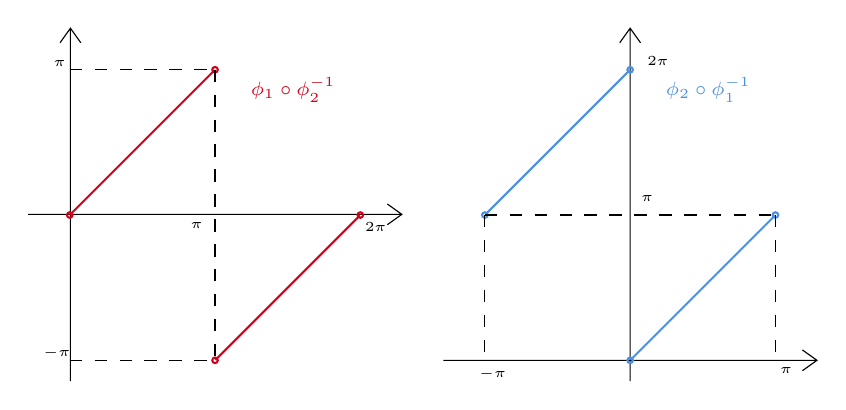
\begin{tikzpicture}[x=0.75pt,y=0.75pt,yscale=-1,xscale=1]
		%uncomment if require: \path (0,300); %set diagram left start at 0, and has height of 300
		
		%Shape: Axis 2D [id:dp031269396086308854] 
		\draw  (180,189.67) -- (360,189.67)(200.33,100) -- (200.33,270) (353,184.67) -- (360,189.67) -- (353,194.67) (195.33,107) -- (200.33,100) -- (205.33,107)  ;
		%Straight Lines [id:da8173483474090752] 
		\draw [color={rgb, 255:red, 208; green, 2; blue, 27 }  ,draw opacity=1 ][line width=0.75]    (200.24,189.76) -- (269.76,120.24) ;
		\draw [shift={(270,120)}, rotate = 315] [color={rgb, 255:red, 208; green, 2; blue, 27 }  ,draw opacity=1 ][line width=0.75]      (0, 0) circle [x radius= 1.34, y radius= 1.34]   ;
		\draw [shift={(200,190)}, rotate = 315] [color={rgb, 255:red, 208; green, 2; blue, 27 }  ,draw opacity=1 ][line width=0.75]      (0, 0) circle [x radius= 1.34, y radius= 1.34]   ;
		%Straight Lines [id:da7972743834901372] 
		\draw [color={rgb, 255:red, 208; green, 2; blue, 27 }  ,draw opacity=1 ][line width=0.75]    (270.24,259.76) -- (339.76,190.24) ;
		\draw [shift={(340,190)}, rotate = 315] [color={rgb, 255:red, 208; green, 2; blue, 27 }  ,draw opacity=1 ][line width=0.75]      (0, 0) circle [x radius= 1.34, y radius= 1.34]   ;
		\draw [shift={(270,260)}, rotate = 315] [color={rgb, 255:red, 208; green, 2; blue, 27 }  ,draw opacity=1 ][line width=0.75]      (0, 0) circle [x radius= 1.34, y radius= 1.34]   ;
		%Straight Lines [id:da11749218813373297] 
		\draw  [dash pattern={on 4.5pt off 4.5pt}]  (270,120) -- (270,260) ;
		%Shape: Axis 2D [id:dp7242837319994968] 
		\draw  (380,260) -- (560,260)(470,100) -- (470,270) (553,255) -- (560,260) -- (553,265) (465,107) -- (470,100) -- (475,107)  ;
		%Straight Lines [id:da7954245800299584] 
		\draw [color={rgb, 255:red, 74; green, 144; blue, 226 }  ,draw opacity=1 ][line width=0.75]    (400.24,189.76) -- (469.76,120.24) ;
		\draw [shift={(470,120)}, rotate = 315] [color={rgb, 255:red, 74; green, 144; blue, 226 }  ,draw opacity=1 ][line width=0.75]      (0, 0) circle [x radius= 1.34, y radius= 1.34]   ;
		\draw [shift={(400,190)}, rotate = 315] [color={rgb, 255:red, 74; green, 144; blue, 226 }  ,draw opacity=1 ][line width=0.75]      (0, 0) circle [x radius= 1.34, y radius= 1.34]   ;
		%Straight Lines [id:da15608839189923596] 
		\draw [color={rgb, 255:red, 74; green, 144; blue, 226 }  ,draw opacity=1 ][line width=0.75]    (470.24,259.76) -- (539.76,190.24) ;
		\draw [shift={(540,190)}, rotate = 315] [color={rgb, 255:red, 74; green, 144; blue, 226 }  ,draw opacity=1 ][line width=0.75]      (0, 0) circle [x radius= 1.34, y radius= 1.34]   ;
		\draw [shift={(470,260)}, rotate = 315] [color={rgb, 255:red, 74; green, 144; blue, 226 }  ,draw opacity=1 ][line width=0.75]      (0, 0) circle [x radius= 1.34, y radius= 1.34]   ;
		%Straight Lines [id:da8863860410352722] 
		\draw  [dash pattern={on 4.5pt off 4.5pt}]  (400,190) -- (400,260) ;
		%Straight Lines [id:da8092780134149673] 
		\draw  [dash pattern={on 4.5pt off 4.5pt}]  (540,190) -- (540,260) ;
		%Straight Lines [id:da9907647632614371] 
		\draw  [dash pattern={on 4.5pt off 4.5pt}]  (400,190) -- (540,190) ;
		%Straight Lines [id:da6719155425075689] 
		\draw  [dash pattern={on 4.5pt off 4.5pt}]  (200,260) -- (270,260) ;
		%Straight Lines [id:da26461137148185054] 
		\draw  [dash pattern={on 4.5pt off 4.5pt}]  (200,120) -- (270,120) ;
		
		% Text Node
		\draw (257,192.4) node [anchor=north west][inner sep=0.75pt]  [font=\tiny]  {$\pi $};
		% Text Node
		\draw (286,122.4) node [anchor=north west][inner sep=0.75pt]  [font=\scriptsize,color={rgb, 255:red, 208; green, 2; blue, 27 }  ,opacity=1 ]  {$\phi _{1} \circ \phi _{2}^{-1}$};
		% Text Node
		\draw (341,192.4) node [anchor=north west][inner sep=0.75pt]  [font=\tiny]  {$2\pi $};
		% Text Node
		\draw (396,262.4) node [anchor=north west][inner sep=0.75pt]  [font=\tiny]  {$-\pi $};
		% Text Node
		\draw (486,122.4) node [anchor=north west][inner sep=0.75pt]  [font=\scriptsize,color={rgb, 255:red, 74; green, 144; blue, 226 }  ,opacity=1 ]  {$\phi _{2} \circ \phi _{1}^{-1}$};
		% Text Node
		\draw (541,262.4) node [anchor=north west][inner sep=0.75pt]  [font=\tiny]  {$\pi $};
		% Text Node
		\draw (474,179.4) node [anchor=north west][inner sep=0.75pt]  [font=\tiny]  {$\pi $};
		% Text Node
		\draw (477,112.4) node [anchor=north west][inner sep=0.75pt]  [font=\tiny]  {$2\pi $};
		% Text Node
		\draw (191,114.4) node [anchor=north west][inner sep=0.75pt]  [font=\tiny]  {$\pi $};
		% Text Node
		\draw (186,252.4) node [anchor=north west][inner sep=0.75pt]  [font=\tiny]  {$-\pi $};
		
		
	\end{tikzpicture}
\end{figure}

\end{solution}

\begin{observation}
	I was thinking about my solution to the problem above, and I thought it is wrong, as I was thinking that the function $ \phi_1 $ is not homeomorphism as it is not continuous. But the point that I was missing is that this function is indeed continuous on its domain and the point of discontinuity (i.e. $ x = \pi $) is not in the domain. 
\end{observation}

\begin{problem}{Another $ C^\infty $ atlas on a circle}
	In the previous problem, we constructed an atlas for a unit circle siting in the complex plane. In this problem we are going to construct a different atlas for a unit circle siting in the $ x-y $ plane. The following diagram are the charts for this unit circle. Write these charts explicitly and check if they are pairwise compatible.
	\begin{figure}[h!]
	
	
	\centering
	\tikzset{every picture/.style={line width=0.75pt}} %set default line width to 0.75pt        
	
	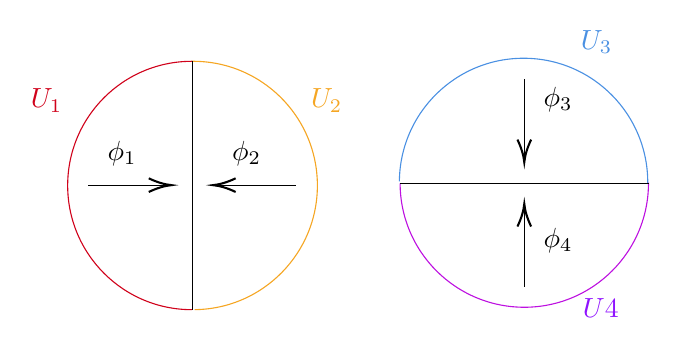
\begin{tikzpicture}[x=0.75pt,y=0.75pt,yscale=-1,xscale=1]
		%uncomment if require: \path (0,300); %set diagram left start at 0, and has height of 300
		
		%Shape: Arc [id:dp023481932229717062] 
		\draw  [draw opacity=0] (199.83,250) .. controls (199.83,250) and (199.83,250) .. (199.83,250) .. controls (199.83,250) and (199.83,250) .. (199.83,250) .. controls (166.79,250) and (140,223.21) .. (140,190.17) .. controls (140,157.12) and (166.79,130.33) .. (199.83,130.33) -- (199.83,190.17) -- cycle ; \draw  [color={rgb, 255:red, 208; green, 2; blue, 27 }  ,draw opacity=1 ] (199.83,250) .. controls (199.83,250) and (199.83,250) .. (199.83,250) .. controls (199.83,250) and (199.83,250) .. (199.83,250) .. controls (166.79,250) and (140,223.21) .. (140,190.17) .. controls (140,157.12) and (166.79,130.33) .. (199.83,130.33) ;  
		%Shape: Arc [id:dp8279857043077765] 
		\draw  [draw opacity=0] (199.83,130.33) .. controls (199.83,130.33) and (199.83,130.33) .. (199.83,130.33) .. controls (232.88,129.98) and (259.95,156.47) .. (260.31,189.52) .. controls (260.67,222.56) and (234.17,249.64) .. (201.13,249.99) -- (200.48,190.16) -- cycle ; \draw  [color={rgb, 255:red, 245; green, 166; blue, 35 }  ,draw opacity=1 ] (199.83,130.33) .. controls (199.83,130.33) and (199.83,130.33) .. (199.83,130.33) .. controls (232.88,129.98) and (259.95,156.47) .. (260.31,189.52) .. controls (260.67,222.56) and (234.17,249.64) .. (201.13,249.99) ;  
		%Shape: Arc [id:dp2277450931666709] 
		\draw  [draw opacity=0] (299.82,188.21) .. controls (299.82,188.21) and (299.82,188.21) .. (299.82,188.21) .. controls (300.08,155.16) and (327.08,128.59) .. (360.13,128.86) .. controls (393.17,129.12) and (419.75,156.12) .. (419.48,189.17) -- (359.65,188.69) -- cycle ; \draw  [color={rgb, 255:red, 74; green, 144; blue, 226 }  ,draw opacity=1 ] (299.82,188.21) .. controls (299.82,188.21) and (299.82,188.21) .. (299.82,188.21) .. controls (300.08,155.16) and (327.08,128.59) .. (360.13,128.86) .. controls (393.17,129.12) and (419.75,156.12) .. (419.48,189.17) ;  
		%Shape: Arc [id:dp16056893747855794] 
		\draw  [draw opacity=0] (419.83,188.83) .. controls (419.83,188.83) and (419.83,188.83) .. (419.83,188.83) .. controls (419.93,221.88) and (393.21,248.74) .. (360.17,248.83) .. controls (327.12,248.93) and (300.26,222.21) .. (300.17,189.17) -- (360,189) -- cycle ; \draw  [color={rgb, 255:red, 189; green, 16; blue, 224 }  ,draw opacity=1 ] (419.83,188.83) .. controls (419.83,188.83) and (419.83,188.83) .. (419.83,188.83) .. controls (419.93,221.88) and (393.21,248.74) .. (360.17,248.83) .. controls (327.12,248.93) and (300.26,222.21) .. (300.17,189.17) ;  
		%Straight Lines [id:da9947609889928073] 
		\draw    (150,190) -- (188,190) ;
		\draw [shift={(190,190)}, rotate = 180] [color={rgb, 255:red, 0; green, 0; blue, 0 }  ][line width=0.75]    (10.93,-3.29) .. controls (6.95,-1.4) and (3.31,-0.3) .. (0,0) .. controls (3.31,0.3) and (6.95,1.4) .. (10.93,3.29)   ;
		%Straight Lines [id:da6553860547904606] 
		\draw    (212,190) -- (250,190) ;
		\draw [shift={(210,190)}, rotate = 0] [color={rgb, 255:red, 0; green, 0; blue, 0 }  ][line width=0.75]    (10.93,-3.29) .. controls (6.95,-1.4) and (3.31,-0.3) .. (0,0) .. controls (3.31,0.3) and (6.95,1.4) .. (10.93,3.29)   ;
		%Straight Lines [id:da19474028508083085] 
		\draw    (360,139) -- (360,177) ;
		\draw [shift={(360,179)}, rotate = 270] [color={rgb, 255:red, 0; green, 0; blue, 0 }  ][line width=0.75]    (10.93,-3.29) .. controls (6.95,-1.4) and (3.31,-0.3) .. (0,0) .. controls (3.31,0.3) and (6.95,1.4) .. (10.93,3.29)   ;
		%Straight Lines [id:da648683487634115] 
		\draw    (360,239) -- (360,201) ;
		\draw [shift={(360,199)}, rotate = 90] [color={rgb, 255:red, 0; green, 0; blue, 0 }  ][line width=0.75]    (10.93,-3.29) .. controls (6.95,-1.4) and (3.31,-0.3) .. (0,0) .. controls (3.31,0.3) and (6.95,1.4) .. (10.93,3.29)   ;
		%Straight Lines [id:da9130830416071034] 
		\draw    (200,130) -- (200,250) ;
		%Straight Lines [id:da1322223309435544] 
		\draw    (420,189) -- (300,189) ;
		
		% Text Node
		\draw (121,142.4) node [anchor=north west][inner sep=0.75pt]  [color={rgb, 255:red, 208; green, 2; blue, 27 }  ,opacity=1 ]  {$U_{1}$};
		% Text Node
		\draw (256,142.4) node [anchor=north west][inner sep=0.75pt]  [color={rgb, 255:red, 245; green, 166; blue, 35 }  ,opacity=1 ]  {$U_{2}$};
		% Text Node
		\draw (386,114.4) node [anchor=north west][inner sep=0.75pt]  [color={rgb, 255:red, 74; green, 144; blue, 226 }  ,opacity=1 ]  {$U_{3}$};
		% Text Node
		\draw (387,243.4) node [anchor=north west][inner sep=0.75pt]  [color={rgb, 255:red, 144; green, 19; blue, 254 }  ,opacity=1 ]  {$U4$};
		% Text Node
		\draw (158,167.4) node [anchor=north west][inner sep=0.75pt]    {$\phi _{1}$};
		% Text Node
		\draw (218,167.4) node [anchor=north west][inner sep=0.75pt]    {$\phi _{2}$};
		% Text Node
		\draw (368,141.4) node [anchor=north west][inner sep=0.75pt]    {$\phi _{3}$};
		% Text Node
		\draw (368,209.4) node [anchor=north west][inner sep=0.75pt]    {$\phi _{4}$};
		
		
	\end{tikzpicture}
\end{figure}

\FloatBarrier
\end{problem}
\begin{solution}
	The explicit formulas for the charts depicted above is as following
	\[ (U_1, \phi_1:U_1\to \R),(U_2, \phi_2:U_2\to \R), (U_3, \phi_3:U_3\to \R),(U_4, \phi_4:U_4\to \R), \]
	where we have
	\[ \phi_1(x,y) = y,\qquad  \phi_2(x,y) = y, \qquad \phi_3(x,y) = x, \qquad \phi_4(x,y) = x. \]
	Note that although some of the functions above might have a same formula, but they are different functions as they have different domains. To show that these functions are pairwise compatible, we start by noting that since $ U_1 \cap U_2 = \emptyset $, thus $ (U_1,\phi_1) $ and $ (U_2,\phi_2) $ are compatible. With the same reasoning, the charts $ (U_3,\phi_3) $ and $ (U_4,\phi_4) $ are compatible. Now, we want to show that $ (U_1,\phi_1) $ is compatible with $ (U_3,\phi_3) $. We need to show that 
	\[ \phi_1 \circ \inv{\phi_3}: \underbrace{\phi_3(U_1\cap U_3)}_{(-1,0)} \to \underbrace{\phi_1(U_1\cap U_3)}_{(0,1)}\quad \text{and} \quad \phi_3\circ \inv{\phi_1}:\underbrace{\phi_1(U_1\cap U_3)}_{(0,1)} \to \underbrace{\phi_3(U_1\cap  U_3)}_{(-1,0)} \]
	are $ C^\infty $. To write them explicitly, we have
	\[ (\phi_1 \circ \inv{\phi_3})(x) = \phi_1(x,\sqrt{1-x^2}) = \sqrt{1-x^2}.  \]
	Also
	\[ (\phi_3 \circ \inv{\phi_1})(x) = \phi_3(-\sqrt{1-x^2},x) = -\sqrt{1-x^2}. \]
	We can see that both of these functions are $ C^\infty $ in their domain. Now, for the charts $ (U_1, \phi_1) $ and $ (U_4,\phi_4) $ need to show
	\[ \phi_1 \circ \inv{\phi_4}:\underbrace{ \phi_4(U_1\cap U_4)}_{(-1,0)} \to \underbrace{\phi_1(U_1\cap U_4)}_{(-1,0)} \qquad \text{and} \qquad \phi_4\circ \inv{\phi_1}: \underbrace{\phi_1(U_1\cap U_4)}_{(-1,0)} \to  \underbrace{\phi_4(U_1\cap U_4)}_{(-1,0)} \]
	are $ C^\infty $ in their domain. Explicitly, we have
	\[ (\phi_1 \circ \inv{\phi_4})(x) = -\sqrt{1 -x^2}, \qquad (\phi_4\circ \inv{\phi_1})(x) = -\sqrt{1-x^2}.\]
	With the same strategy, we can show that this collection of charts indeed makes a $ C^\infty $ atlas for the unit circle in $ x-y $ plane.
\end{solution}


\begin{problem}[The real line with two origins (from W. Tu)]
	Let $ A $ and $ B $ be two points not on the real line $ \R $. Consider the set $ S = (\R - \set{0}) \cup \set{A,B} $. For nay two positive real numbers $ c,d $, define 
	\[ I_A(-c,d) = (-c,0) \cup \set{A} \cap (0,d) \]
	and similarly for $ I_B(-c,d) $, with $ B $ instead of $ A $. Define a topology on $ S $ as follows: On $ (\R - \set{0}) $, use the subspace topology inherited from $ \R $, with open intervals as a basis. A basis of neighborhoods at $ A $ is the set $ \set{I_A(-c,d)\ |\ c,d > 0} $; similarly, a basis of neighborhoods at $ B $ is $ \set{I_B(-c,d)\ |\ c,d > 0} $.
	\begin{enumerate}[(a)]
		\item Prove that the map $ h: I_A(-c,d) \to (-c,d) $ defined by
		\begin{align*}
			h(x)&=x \qquad \text{for}\ x\in(-c,0) \cup (0,d),\\
			h(A)&=0
		\end{align*}
		is a homeomorphism.
		
		\item Show that $ S $ is locally Euclidean and second countable, but not Hausdorff.
	\end{enumerate}
\end{problem}

\begin{solution}
	\begin{enumerate}[(a)]
		\item We need to show that $ h $ is one-to-one, onto, and continuous, with continuous inverse. To show being one-to-one, let $ x,y \in I_A(-c,d) $ such that $ x\neq y $ and possibly one of them equal to $ A $. If none is equal to $ A $, then $ h $ is the identity map which is one-to-one. However, if one of them is equal to $ A $, let's say $ x = A $, then $ h(x) = 0 $ where $ h(y) \in (-c,d)\cup(0,d)$, thus $ h(y) \neq 0 $. This proves that $ h $ is indeed one to one. To show that the function is onto, let $ z \in (-c,d) $. Then if $ z = 0 $ we have $ h(A) = z $, and if $ z \neq 0 $, we have $ h(z) = z $. Thus the function $ h $ is a bijection.
		
		As the second step, we need to show that this function is continuous with continuous inverse. From definition of continuoity, we just need to show that both $ h $ and $ \inv{h} $ maps opens to opens (because for continuous function the pre-image of every open set is an open set; and to show that the inverse of the function is also continuous we need to show that the image of every open is also open).
		Let $ U = (a,b) \subset I_A(-c,d) $ be an open set in the topology of $ S $. If $ A \notin (a,b) $, then the image of this set under $ h $ is $ (a,b) $ which is open in $ (-c,d) $. But if $ A \in (a,b) $, then the image of this set under the map $ h $ is $ (a,0)\cup(0,b)\cup\set{0} = (a,b) $, which is also open. Thus $ \inv{h} $ is continuous. To show the continuity of $ \inv{h} $, let $ (a,b) \subset (c,d) $. If $ 0 \notin (a,b) $, then pre-image of this set under the map $ f $ is $ (a,b) $ that is open in $ S $. However if $ 0 \in (a,b) $, then the pre-image of this set under $ f $ is the set $ (-a,0) \cup \set{A} \cup (0,b) $ which is indeed open in $ S $ as we can construct this with the basis if opens at $ A $.
		
		\item First, we show that $ S $ is locally Euclidean. To show this let $ p \in S $. If $ p \neq A $ and $ p \neq B $, then we choose an open set $ U =  (a,b) $ containing $ p $ that does not contain neither of $ A $ and  $ B $. Then $ U $ is homeomorphic to $ (a,b) $ with the identity map. However if $ p = A $, we choose any open $ U = (a,b) $ containing $ p $. Then $ (U = (a,b),I_A(a,b)) $ is a local chart. For the case where $ p = B $, we can find a suitable chart with the same reasoning as for $ A $. Thus we have shown that $ S $ is locally Euclidean.
		
		To show that $ S $ is second countable, let $ \mathcal{B} $ be a basis for $ \R - \set{0} $. Since $ \R $ is second countable, then $ \mathcal{B} $ is countable. Let $ \mathbb{B} = \mathcal{B} \cup I_A(-c,d) \cup I_B(-c,d) $ is a countable basis for $ S $ for some $ c,d > 0 $. This shows that $ S $ is also second countable.
		
		However, this space is not Hausdorff. To show this consider the points $ A,B $. We can not find any two open $ U,V $ such that $ A \in U $ and $ B \in V $ and we have $ U \cap V = \emptyset $. Or equivalently, for all open sets $ U,V $  such that $ A \in U $ and $ B \in V $ we have $ U\cap V \neq \emptyset $. That is because from the basis of the open neighborhoods at $ A,B $ we have $ U = I_A(-c,d) $ and $ V = I_B(-e,f) $ for some $ c,d,e,f > 0 $. It is clear that $ U \cap V \neq 0 $, thus $ S $ is not Hausdorff.
	\end{enumerate}
\end{solution}

\begin{problem}[A sphere with a hair (from W. Tu) ] 
	A fundamental theorem of topology, the theorem on invariance of dimension, states that if two nonempty open sets $ U \subset \R^n $ and $ V \subset \R^m $ are homeomorphic, then $ n = m $. Prove that the sphere with a hair in $ \R^3 $ is not locally Euclidean at $ q $ (the point that the hair attaches to the sphere). Hence it cannot be a topological manifold. 
\end{problem}

\begin{solution}
	We will proceed with the proof by contradiction. Assume that the ball with hair at  point $ q $ is homeomorphic to some open set in $ \R^n $. Then $ q $ has an open neighborhood $ U $ homeomorphic to an open ball $ B := \mathbb{B}(0,\epsilon) \in \R^n $, with $ q $ mapping to 0. We can restrict this homeomorphism to a homeomorphism $ U - \set{q} \to B - \set{0} $. Now $ B-\set{0} $ is either connected if $ n \geq 2 $ or has two connected components if $ n=1 $, where $ U - \set{q} $ has two connected components where one component is a 1 dimensional manifold (the hair) and the other component is a 2 dimensional manifold (the sphere). The only case where $ B - \set{0} $ has two connected components is when $ n = 1 $. But because of the invariance of dimension principle, the sphere (2 dimensional manifold) can not be homeomorphic to a one dimensional manifold. Thus there is no such a homeomorphism between the hairy ball and $ \R^n $ and the hairy ball is not locally Euclidean in $ q $.
\end{solution}

\begin{problem}[Charts on a sphere (from W. Tu)]
	Let $ S^2 $ be the unit sphere, i.e.
	\[ S^2 = \set{(x,y,z)\in\R^3\ :\ x^2+y^2+z^2 = 1} \]
	in $ \R^3 $. Define in $ S^2 $ the six charts corresponding to the six hemispheres (from the front, rear, right, left, upper, and lower hemispheres) as in the figure.
	\begin{align*}
		U_1 = \set{(x,y,z) \in S^2\ |\ x > 0}, \qquad \phi_1(x,y,z) = (y,z), \\
		U_2 = \set{(x,y,z) \in S^2\ |\ x < 0}, \qquad \phi_2(x,y,z) = (y,z), \\
		U_3 = \set{(x,y,z) \in S^2\ |\ y > 0}, \qquad \phi_3(x,y,z) = (x,z), \\
		U_4 = \set{(x,y,z) \in S^2\ |\ y < 0}, \qquad \phi_4(x,y,z) = (x,z), \\
		U_5 = \set{(x,y,z) \in S^2\ |\ z > 0}, \qquad \phi_5(x,y,z) = (x,y), \\
		U_6 = \set{(x,y,z) \in S^2\ |\ z < 0}, \qquad \phi_6(x,y,z) = (x,y).
	\end{align*}
	Note that although some of the functions above might look similar (like $ \phi_3 $ and $ \phi_4 $) but they are in fact different functions as they have different domains. Show that $ \phi_1\circ \inv{\phi_4}, \phi_4 \circ \inv{\phi_1} $ is $ C^\infty $ on $ \phi_4(U_1 \cap U_4), \phi_1(U_1 \cap U_4) $ respectively. Do the same same analysis for $ \phi_6 \circ \inv{\phi_1}$.
	\begin{figure}[h!]
	
	\centering
	
	\tikzset{every picture/.style={line width=0.75pt}} %set default line width to 0.75pt        
	
	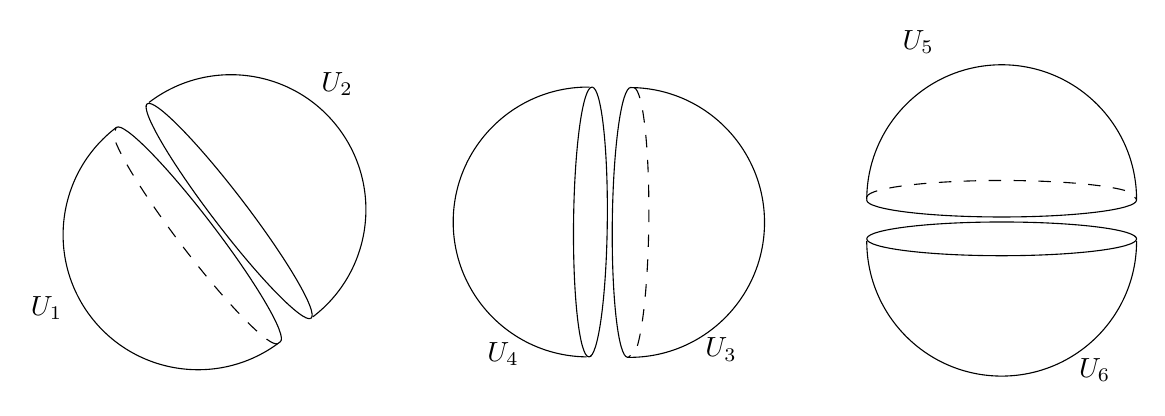
\begin{tikzpicture}[x=0.75pt,y=0.75pt,yscale=-1,xscale=1]
		%uncomment if require: \path (0,300); %set diagram left start at 0, and has height of 300
		
		%Shape: Arc [id:dp8087392079745468] 
		\draw  [draw opacity=0] (610,205) .. controls (610,205) and (610,205) .. (610,205) .. controls (610,240.9) and (580.9,270) .. (545,270) .. controls (509.1,270) and (480,240.9) .. (480,205) -- (545,205) -- cycle ; \draw   (610,205) .. controls (610,205) and (610,205) .. (610,205) .. controls (610,240.9) and (580.9,270) .. (545,270) .. controls (509.1,270) and (480,240.9) .. (480,205) ;  
		%Shape: Arc [id:dp7144643582066421] 
		\draw  [draw opacity=0] (480.02,203.67) .. controls (480.89,199.28) and (509.65,195.75) .. (545,195.75) .. controls (578.58,195.75) and (606.22,198.93) .. (609.64,203.02) -- (545,203.88) -- cycle ; \draw   (480.02,203.67) .. controls (480.89,199.28) and (509.65,195.75) .. (545,195.75) .. controls (578.58,195.75) and (606.22,198.93) .. (609.64,203.02) ;  
		%Shape: Arc [id:dp9774877190814104] 
		\draw  [draw opacity=0] (480,185) .. controls (480,185) and (480,185) .. (480,185) .. controls (480,149.1) and (509.1,120) .. (545,120) .. controls (580.9,120) and (610,149.1) .. (610,185) -- (545,185) -- cycle ; \draw   (480,185) .. controls (480,185) and (480,185) .. (480,185) .. controls (480,149.1) and (509.1,120) .. (545,120) .. controls (580.9,120) and (610,149.1) .. (610,185) ;  
		%Shape: Arc [id:dp7118645098131682] 
		\draw  [draw opacity=0] (609.09,202.51) .. controls (609.69,202.95) and (610,203.41) .. (610,203.88) .. controls (610,208.36) and (580.9,212) .. (545,212) .. controls (509.1,212) and (480,208.36) .. (480,203.88) .. controls (480,203.8) and (480.01,203.73) .. (480.02,203.66) -- (545,203.88) -- cycle ; \draw   (609.09,202.51) .. controls (609.69,202.95) and (610,203.41) .. (610,203.88) .. controls (610,208.36) and (580.9,212) .. (545,212) .. controls (509.1,212) and (480,208.36) .. (480,203.88) .. controls (480,203.8) and (480.01,203.73) .. (480.02,203.66) ;  
		%Shape: Arc [id:dp7962209595423704] 
		\draw  [draw opacity=0] (609.06,183.85) .. controls (609.66,184.29) and (609.98,184.75) .. (609.98,185.22) .. controls (609.98,189.7) and (580.88,193.34) .. (544.98,193.34) .. controls (509.08,193.34) and (479.98,189.7) .. (479.98,185.22) .. controls (479.98,185.14) and (479.99,185.07) .. (480,185) -- (544.98,185.22) -- cycle ; \draw   (609.06,183.85) .. controls (609.66,184.29) and (609.98,184.75) .. (609.98,185.22) .. controls (609.98,189.7) and (580.88,193.34) .. (544.98,193.34) .. controls (509.08,193.34) and (479.98,189.7) .. (479.98,185.22) .. controls (479.98,185.14) and (479.99,185.07) .. (480,185) ;  
		%Shape: Arc [id:dp26854896682720364] 
		\draw  [draw opacity=0][dash pattern={on 4.5pt off 4.5pt}] (480.02,183.67) .. controls (480.89,179.28) and (509.65,175.75) .. (545,175.75) .. controls (578.58,175.75) and (606.22,178.93) .. (609.64,183.02) -- (545,183.88) -- cycle ; \draw  [dash pattern={on 4.5pt off 4.5pt}] (480.02,183.67) .. controls (480.89,179.28) and (509.65,175.75) .. (545,175.75) .. controls (578.58,175.75) and (606.22,178.93) .. (609.64,183.02) ;  
		%Shape: Arc [id:dp8593027572319052] 
		\draw  [draw opacity=0] (345,260.74) .. controls (345,260.74) and (345,260.74) .. (345,260.74) .. controls (345,260.74) and (345,260.74) .. (345,260.74) .. controls (309.1,260.33) and (280.34,230.89) .. (280.75,195) .. controls (281.16,159.1) and (310.6,130.34) .. (346.49,130.75) -- (345.74,195.74) -- cycle ; \draw   (345,260.74) .. controls (345,260.74) and (345,260.74) .. (345,260.74) .. controls (345,260.74) and (345,260.74) .. (345,260.74) .. controls (309.1,260.33) and (280.34,230.89) .. (280.75,195) .. controls (281.16,159.1) and (310.6,130.34) .. (346.49,130.75) ;  
		%Shape: Arc [id:dp5017110012711772] 
		\draw  [draw opacity=0] (347.82,130.78) .. controls (352.2,131.7) and (355.4,160.5) .. (354.99,195.85) .. controls (354.61,229.43) and (351.11,257.03) .. (346.98,260.41) -- (346.87,195.76) -- cycle ; \draw   (347.82,130.78) .. controls (352.2,131.7) and (355.4,160.5) .. (354.99,195.85) .. controls (354.61,229.43) and (351.11,257.03) .. (346.98,260.41) ;  
		%Shape: Arc [id:dp34022749055732393] 
		\draw  [draw opacity=0] (366.49,130.98) .. controls (366.49,130.98) and (366.49,130.98) .. (366.49,130.98) .. controls (402.39,131.39) and (431.15,160.83) .. (430.74,196.72) .. controls (430.33,232.62) and (400.89,261.38) .. (364.99,260.97) -- (365.74,195.97) -- cycle ; \draw   (366.49,130.98) .. controls (366.49,130.98) and (366.49,130.98) .. (366.49,130.98) .. controls (402.39,131.39) and (431.15,160.83) .. (430.74,196.72) .. controls (430.33,232.62) and (400.89,261.38) .. (364.99,260.97) ;  
		%Shape: Arc [id:dp9156415467589833] 
		\draw  [draw opacity=0] (347.5,259.86) .. controls (347.05,260.45) and (346.59,260.76) .. (346.12,260.75) .. controls (341.63,260.7) and (338.33,231.56) .. (338.74,195.66) .. controls (339.16,159.77) and (343.13,130.71) .. (347.62,130.76) .. controls (347.69,130.76) and (347.76,130.77) .. (347.83,130.79) -- (346.87,195.76) -- cycle ; \draw   (347.5,259.86) .. controls (347.05,260.45) and (346.59,260.76) .. (346.12,260.75) .. controls (341.63,260.7) and (338.33,231.56) .. (338.74,195.66) .. controls (339.16,159.77) and (343.13,130.71) .. (347.62,130.76) .. controls (347.69,130.76) and (347.76,130.77) .. (347.83,130.79) ;  
		%Shape: Arc [id:dp7534866185784517] 
		\draw  [draw opacity=0] (366.15,260.05) .. controls (365.7,260.64) and (365.24,260.95) .. (364.78,260.95) .. controls (360.29,260.89) and (356.99,231.75) .. (357.4,195.86) .. controls (357.82,159.96) and (361.79,130.9) .. (366.28,130.95) .. controls (366.35,130.96) and (366.42,130.96) .. (366.49,130.98) -- (365.53,195.95) -- cycle ; \draw   (366.15,260.05) .. controls (365.7,260.64) and (365.24,260.95) .. (364.78,260.95) .. controls (360.29,260.89) and (356.99,231.75) .. (357.4,195.86) .. controls (357.82,159.96) and (361.79,130.9) .. (366.28,130.95) .. controls (366.35,130.96) and (366.42,130.96) .. (366.49,130.98) ;  
		%Shape: Arc [id:dp7058755896129407] 
		\draw  [draw opacity=0][dash pattern={on 4.5pt off 4.5pt}] (367.82,131.01) .. controls (372.2,131.93) and (375.4,160.73) .. (374.99,196.08) .. controls (374.61,229.66) and (371.1,257.26) .. (366.98,260.64) -- (366.87,195.99) -- cycle ; \draw  [dash pattern={on 4.5pt off 4.5pt}] (367.82,131.01) .. controls (372.2,131.93) and (375.4,160.73) .. (374.99,196.08) .. controls (374.61,229.66) and (371.1,257.26) .. (366.98,260.64) ;  
		%Shape: Arc [id:dp6580687340920708] 
		\draw  [draw opacity=0] (134.21,138.15) .. controls (134.21,138.15) and (134.21,138.15) .. (134.21,138.15) .. controls (134.21,138.15) and (134.21,138.15) .. (134.21,138.15) .. controls (162.73,116.35) and (203.52,121.79) .. (225.32,150.31) .. controls (247.13,178.82) and (241.69,219.62) .. (213.17,241.42) -- (173.69,189.79) -- cycle ; \draw   (134.21,138.15) .. controls (134.21,138.15) and (134.21,138.15) .. (134.21,138.15) .. controls (134.21,138.15) and (134.21,138.15) .. (134.21,138.15) .. controls (162.73,116.35) and (203.52,121.79) .. (225.32,150.31) .. controls (247.13,178.82) and (241.69,219.62) .. (213.17,241.42) ;  
		%Shape: Arc [id:dp04807301977746614] 
		\draw  [draw opacity=0] (212.1,242.21) .. controls (208.08,244.19) and (187.81,223.49) .. (166.34,195.4) .. controls (145.94,168.73) and (131.69,144.84) .. (132.85,139.64) -- (172.79,190.47) -- cycle ; \draw   (212.1,242.21) .. controls (208.08,244.19) and (187.81,223.49) .. (166.34,195.4) .. controls (145.94,168.73) and (131.69,144.84) .. (132.85,139.64) ;  
		%Shape: Arc [id:dp5373023961242778] 
		\draw  [draw opacity=0] (197.28,253.57) .. controls (197.28,253.57) and (197.28,253.57) .. (197.28,253.57) .. controls (197.28,253.57) and (197.28,253.57) .. (197.28,253.57) .. controls (168.76,275.37) and (127.97,269.93) .. (106.16,241.41) .. controls (84.36,212.89) and (89.8,172.1) .. (118.32,150.3) -- (157.8,201.93) -- cycle ; \draw   (197.28,253.57) .. controls (197.28,253.57) and (197.28,253.57) .. (197.28,253.57) .. controls (197.28,253.57) and (197.28,253.57) .. (197.28,253.57) .. controls (168.76,275.37) and (127.97,269.93) .. (106.16,241.41) .. controls (84.36,212.89) and (89.8,172.1) .. (118.32,150.3) ;  
		%Shape: Arc [id:dp6075301311311689] 
		\draw  [draw opacity=0] (132.79,140.39) .. controls (132.77,139.64) and (132.95,139.11) .. (133.31,138.83) .. controls (136.88,136.11) and (157.44,157.02) .. (179.25,185.53) .. controls (201.05,214.05) and (215.84,239.38) .. (212.27,242.11) .. controls (212.22,242.15) and (212.15,242.19) .. (212.09,242.22) -- (172.79,190.47) -- cycle ; \draw   (132.79,140.39) .. controls (132.77,139.64) and (132.95,139.11) .. (133.31,138.83) .. controls (136.88,136.11) and (157.44,157.02) .. (179.25,185.53) .. controls (201.05,214.05) and (215.84,239.38) .. (212.27,242.11) .. controls (212.22,242.15) and (212.15,242.19) .. (212.09,242.22) ;  
		%Shape: Arc [id:dp4893987696896971] 
		\draw  [draw opacity=0] (117.98,151.74) .. controls (117.96,150.99) and (118.14,150.47) .. (118.5,150.18) .. controls (122.07,147.46) and (142.64,168.37) .. (164.44,196.89) .. controls (186.24,225.4) and (201.03,250.73) .. (197.46,253.46) .. controls (197.41,253.5) and (197.34,253.54) .. (197.28,253.57) -- (157.98,201.82) -- cycle ; \draw   (117.98,151.74) .. controls (117.96,150.99) and (118.14,150.47) .. (118.5,150.18) .. controls (122.07,147.46) and (142.64,168.37) .. (164.44,196.89) .. controls (186.24,225.4) and (201.03,250.73) .. (197.46,253.46) .. controls (197.41,253.5) and (197.34,253.54) .. (197.28,253.57) ;  
		%Shape: Arc [id:dp5010740042347757] 
		\draw  [draw opacity=0][dash pattern={on 4.5pt off 4.5pt}] (196.21,254.36) .. controls (192.19,256.34) and (171.92,235.64) .. (150.45,207.55) .. controls (130.05,180.87) and (115.8,156.99) .. (116.96,151.78) -- (156.91,202.62) -- cycle ; \draw  [dash pattern={on 4.5pt off 4.5pt}] (196.21,254.36) .. controls (192.19,256.34) and (171.92,235.64) .. (150.45,207.55) .. controls (130.05,180.87) and (115.8,156.99) .. (116.96,151.78) ;  
		
		% Text Node
		\draw (76,230.4) node [anchor=north west][inner sep=0.75pt]    {$U_{1}$};
		% Text Node
		\draw (216,122.4) node [anchor=north west][inner sep=0.75pt]    {$U_{2}$};
		% Text Node
		\draw (401,250.4) node [anchor=north west][inner sep=0.75pt]    {$U_{3}$};
		% Text Node
		\draw (296,252.4) node [anchor=north west][inner sep=0.75pt]    {$U_{4}$};
		% Text Node
		\draw (496,102.4) node [anchor=north west][inner sep=0.75pt]    {$U_{5}$};
		% Text Node
		\draw (581,260.4) node [anchor=north west][inner sep=0.75pt]    {$U_{6}$};
		
		
	\end{tikzpicture}
\end{figure}
\end{problem}
\begin{solution}
	For the set $ U_1 \cap U_4 $ we have
	\[ U_1 \cap U_4 = \set{(x,y,z) \in S^2\ :\ x>0 \text{ and } y < 0 }. \]
	Thus we will have
	\[ \phi_4(U_1\cap U_4) = \set{(x,z)\in \R^2 \ :\ x^2 + z^2 \leq 1,\ x>0}. \]
	Thus we can write
	\[ (\phi_1 \circ \inv{\phi_4})(\langle x,z \rangle ) = \phi_1(\langle x,-\sqrt{1-(x^2+y^2)},z \rangle) = \langle -\sqrt{1-(x^2+y^2)},z \rangle  \]
	This is indeed a $ C^\infty $ vector valued function, since each component is a $ C^\infty $ function. Now to evaluate $ \phi_4 \circ \inv{\phi_1}: \phi_1(U_1 \cap U_4) \to \phi_4(U_1\cap U_4) $ we need to first evaluate the set $ \phi_1(U_1 \cap U_4) $. For this set we have
	\[ \phi_1(U_1 \cap U_4) = \set{(z,y)\in\R^2\ :\ z^2 + y^2 \leq 1, y < 0}. \]
	Then we can write
	\[ (\phi_4 \circ \inv{\phi_1})(\langle y,z \rangle ) = \phi_4(\langle \sqrt{1-(y^2+z^2)}, y,z  \rangle) = \langle \sqrt{1-(y^2+z^2)} , z \rangle. \]
	This is indeed a $ C^\infty $ vector valued function. 
	
	To evaluate the function $ \phi_6 \circ \inv{\phi}_1: \phi_1(U_1 \cap U_6) \to \phi_6(U_1 \cap U_6) $, we first need to determine the domain of this function. First observe that 
	\[ U_1 \cap U_6 =  \set{(x,y,z) \in S^2\ :\ x>0 \text{ and } y<0}, \]
	which is the same as $ U_1 \cap U_4 $. Then for the domain of the function of interest we can write
	\[ \phi_1(U_1 \cap U_6) = \set{(y,z) \in \R^2 :\ z^2 + y^2 \leq 1 \text{ and } y<0}, \]
	\[ (\phi_6 \circ \inv{\phi_1})(\langle y,z \rangle) = \phi_6(\langle \sqrt{1-(y^2+z^2)},y,z \rangle) = \langle \sqrt{1-(y^2+z^2)}, y \rangle. \]
\end{solution}

\begin{problem}[Existence of a coordinate neighborhood (from W. Tu)]
	Let $ \set{(U_\alpha, \phi_\alpha)}_{\alpha \in I} $ be the maximal atlas on manifold $ M $. For any open set $ U $ in $ M $ and a point $ p \in U $, prove the existence of a coordinate open set $ U_\alpha $ such that $ p \in U_\alpha \subset U $.
\end{problem}
\begin{solution}
	Since $ \set{(U_\alpha,\phi_\alpha)}_{\alpha \in I} $ is an atlas, then for $ p \in U $ given as above, we can find some $ \alpha_1 \in I $ such that $ p \in U_{\alpha_1} $. Consider the open set $ W = U_{\alpha_1} \cap U $. The chart $ (W, \phi_{\alpha_1}|_W) $ is in the atlas (since it is maximal), i.e. $ \exists \alpha \in I $ such that $ (U_\alpha, \phi_\alpha) = (W, \phi_{\alpha_1}|_W) $. This completes the proof.
\end{solution}

\begin{problem}[An atlas for a product manifold (from W. Tu)]
	Prove the following proposition.
	\begin{proposition}
		If $ \set{(U_\alpha,\phi_\alpha)} $ and $ \set{(V_i,\psi_i)} $ are $ C^\infty $ atlases for the manifold $ M $ and $ N $ of dimensions $ m $ and $ n $, respectively, then the collection 
		\[ \set{(U_\alpha \times V_i,\phi_\alpha \times \psi_i)} \] where
		\[ \phi_\alpha \times \psi_i\ :\ U_\alpha \times V_i \to \R^m \times \R^n \]
		of charts is a $ C^\infty $ atlas on $ M\times N $. Therefore, $ M\times N $ is a $ C^\infty $ manifold of dimension $ m+n $.
	\end{proposition}
\end{problem}
\begin{solution}
	In order to show that the collection $ \frak{U} = \set{(U_\alpha \times V_i, \phi_\alpha \times \psi_i)} $ is an atlas for $ M\times N $, we need to show that charts are pairwise compatible as well as the set covering the whole space. To show that the chart covers the whole space $ M\times N $, let $ (p_1,p_2) \in M\times N $. Then $ p_1 \in M $ and $ p_2 \in N $. Then there are two coordinate open sets such that $ p_1 \in U_{\alpha_1} $ and $ p_2 \in V_{i_1} $. Thus the coordinate open set $ U_{\alpha_1} \times V_{i_1} $ contains the point $ (p_1,p_2) $.
	
	To show that two any two charts in the collection $ \frak{U} $ are compatible, let $ (U_{\alpha_1} \times V_{i_1},\phi_{\alpha_1}\times \psi_{i_1}) $ and $  (U_{\alpha_2} \times V_{i_2},\phi_{\alpha_2}\times \psi_{i_2}) $ be two  charts. We claim that the corresponding coordinate maps are $ C^\infty $. This follows directly from the fact the each component of the map these coordinate maps are $ C^\infty $.
\end{solution}





\end{document}